% 必要な項目ができた場合は適宜サブセクションを追加してください
%\include{begin}

% イベント名を記入する
\section{朝の集い}

% 日時と場所を記入する
% 時刻は4桁で記入すること!
\subsection{日時・場所}
\begin{tabular}{p{2zw}rp{38zw}}
  日時 & : & 2019年4月6日(土) 06:30 $\sim$ 07:45\\
  場所 & : & 正面広間(雨天中止) \\
\end{tabular}

% 目的を記入する
\subsection{目的}
規則正しい生活を実現し,国旗・所旗が掲揚されていくと同時に本日の活動を再確認し,心身共々健康になる.

\subsection{タイムスケジュール(晴天時)}
% イベントのタイムスケジュールを記入する
% 時刻は必ず4桁(00:00)で記入すること!
% 時間の流れは途切れないように記述する!
\begin{longtable}{p{3zw}p{39zw}}
  06:35 & \textbf{◎ 移動開始} \\
        & \ \ \textbullet \ \ 整列係(???, ???)は新入生の誘導開始前に正面広間に移動し,整列の準備をする\\
        & \ \ \textbullet \ \ 誘導係(???,???,???,???,???, ???,???,???)は宿泊棟から誘導を開始する \\
        & \ \ \textbullet \ \ ???,???,???,???は誘導開始時に報告slackに報告する \\
        & \ \ \textbullet \ \ その他のスタッフは正面広間に到着後,誘導係(???,???,???,???,???,???,???,???),整列係(???,???)の指示に従って新入生を並ばせる\\\\

  06:50 & \textbf{◎ 国旗・施設旗掲揚 ラジオ体操 スタッフ代表の挨拶} \\
        & \ \ \textbullet \ \ 幡多職員の指示に従い,国旗・施設旗掲揚,ラジオ体操(???, ???),スタッフ代表(???)の挨拶を行う \\
        & \ \ \textbullet \ \ イベント準備スタッフ(???,???,???,???)は朝の集いが始まる頃に食堂に移動し,朝食をとる \\
        & \ \ \textbullet \ \ 朝食時の食堂内誘導スタッフ(???, ???,???)は,朝の集いの終わり頃に食堂へ移動しやすい場所で待機する \\
        & \ \  ※???は前日の野外炊事に国旗・所旗掲揚する新入生2名を見つけて交渉しておく \\\\

  07:00 & \textbf{◎ 食堂へ移動開始} \\
        & \ \ \textbullet \ \ ???は挨拶終了後,アレルギーを持っている新入生は正面広間に残り,それ以外の新入生は食堂へ移動するように指示し,報告slackに食堂へ誘導開始の旨を報告する \\
        & \ \ \textbullet \ \ ???は(事前に顔を見て名前と一致させておくこと)アレルギーを持っている新入生に対して,朝食・昼食をとる際の注意事項(事前に調べておく)を伝え(るが食事の変更は無い),食堂に移動する \\
        & \ \ \textbullet \ \ 最初に教職員から食堂へ行って頂くため,先生誘導係(???,???)は食堂までの誘導を行う(新入生は待機) \\
        & \ \ \textbullet \ \ 食堂内誘導スタッフ(???,???,???)も急いで食堂に向かい,食堂内の各々のポジションに配置し,新入生が入ってきたら,奥から詰めて座ることを伝える \\
        & \ \ \textbullet \ \ 宿泊棟から正面広間への誘導係(???, ???,???,???,???,???)と正面広間から食堂までの誘導係(???, ???, ???)は食堂へ誘導を行う \\
        & \ \ \textbullet \ \ ???を先頭に食堂への誘導を開始し,???はトイレに行きたい新入生がいたら連れて行く \\ %(トイレは浴場横のものを使用する)
        & \ \ \textbullet \ \ ???は新入生の列の中間あたりで誘導を行い,食堂に着き次第,食堂内での誘導を行う \\
        & \ \ \textbullet \ \ 各スタッフも誘導しながら,奥からつめて座るように指示する \\
        & \ \ \textbullet \ \ ???は新入生の最後尾について全員の移動を確認する \\\\

  07:45 & \textbf{◎ 食堂への移動完了} \\
        & \ \ \textbullet \ \ ???は全員が食堂に入り終えたら報告slackに報告する(???が新入生をトイレに誘導していないかも確認) \\\\
\end{longtable}


\subsection{タイムスケジュール(雨天時)}
\begin{longtable}{p{3zw}p{39zw}}
  06:35 & \textbf{◎ 移動開始} \\
        & \ \ \textbullet \ \ 整列係(???, ???)は新入生の誘導開始前に大研修室に移動し,整列の準備をする\\
        & \ \ \textbullet \ \ 誘導係(???,???,???,???,???, ???,???,???)は宿泊棟から誘導を開始する \\
        & \ \ \textbullet \ \ ???,???,???,???は誘導開始時に報告slackに報告する \\
        & \ \ \textbullet \ \ その他のスタッフは大研修室に到着後,誘導係(???,???,???,???,???,???,???,???),整列係(???,???)の指示に従って新入生を並ばせる\\\\

  06:50 & \textbf{◎ スタッフ代表の挨拶} \\
        & \ \ \textbullet \ \ 幡多職員の指示に従い,スタッフ代表(???)の挨拶を行う \\
        & \ \ \textbullet \ \ イベント準備スタッフ(???,???,???,???)は朝の集いが始まる頃に食堂に移動し,朝食をとる \\
        & \ \ \textbullet \ \ 朝食時の食堂内誘導スタッフ(???, ???,???)は,朝の集いの終わり頃に食堂へ移動しやすい場所で待機する \\

  07:00 & \textbf{◎ 食堂へ移動開始} \\
        & \ \ \textbullet \ \ ???は挨拶終了後,アレルギーを持っている新入生はその場に残り,それ以外の新入生は食堂へ移動するように指示し,報告slackに食堂へ誘導開始の旨を報告する \\
        & \ \ \textbullet \ \ ???は(事前に顔を見て名前と一致させておくこと)アレルギーを持っている新入生に対して,朝食・昼食をとる際の注意事項(事前に調べておく)を伝え(るが食事の変更は無い),食堂に移動する \\
        & \ \ \textbullet \ \ 最初に教職員から食堂へ行って頂くため,先生誘導係(???,???)は食堂までの誘導を行う(新入生は待機) \\
        & \ \ \textbullet \ \ 食堂内誘導スタッフ(???,???,???)も急いで食堂に向かい,食堂内の各々のポジションに配置し,新入生が入ってきたら,奥から詰めて座ることを伝える \\
        & \ \ \textbullet \ \ 宿泊棟から正面広間への誘導係(???, ???,???,???,???,???)と正面広間から食堂までの誘導係(???, ???, ???)は食堂へ誘導を行う \\
        & \ \ \textbullet \ \ 食堂への誘導を開始し,???はトイレに行きたい新入生がいたら連れて行く \\ %(トイレは浴場横のものを使用する)
        & \ \ \textbullet \ \ 各スタッフは誘導しながら,奥からつめて座るように指示する \\
        & \ \ \textbullet \ \ ???は新入生の最後尾について全員の移動を確認する \\\\

 07:10  & \textbf{◎ 食堂への移動完了} \\
       & \ \ \textbullet \ \ 食堂内スタッフ(???)は入り口で誘導を行い,全員が食堂に入り終えたら報告slackに報告する \\\\
\end{longtable}


% イベントに必要な役割と人数を記入する
% 担当者は決定次第追記する
% 記入例 ・司会者 2人(名前1、名前2)
\subsection{人員配置}
◎晴天時
\begin{itemize}
\item くろしお棟1から正面広間への誘導係:日下,松尾
\item くろしお棟2から正面広間への誘導係:立岩,松林
\item くろしお棟3から正面広間への誘導係:平松,宮尾
\item くろしお棟4から正面広間への誘導係:高橋(錬),小野
\item 整列係:小谷,渡辺
\item ラジオ体操のお兄さん:藤沢,宮尾
\item 旗揚げ係:松林 角原 野外炊事に上村がスカウトした新入生2名
\item スタッフ代表の挨拶:以西
\item 正面広間から食堂までの誘導係:下出,高島,小松
\item 食堂内での誘導係:南部,高橋(果),別役
\item イベント準備スタッフ:横田,長道,野田,和田
\end{itemize}
◎雨天時
\begin{itemize}
\item くろしお棟1から食堂への誘導係:日下,松尾
\item くろしお棟2から食堂への誘導係:立岩,松林
\item くろしお棟3から食堂への誘導係:平松,宮尾
\item くろしお棟4から正面広間への誘導係:高橋(錬),小野
\item イベント準備スタッフ:横田,長道,野田,和田
\item 食堂内誘導スタッフ:南部,高橋(果),別役

\end{itemize}



\subsection{全体配置}
\begin{figure}[h]
\begin{center}
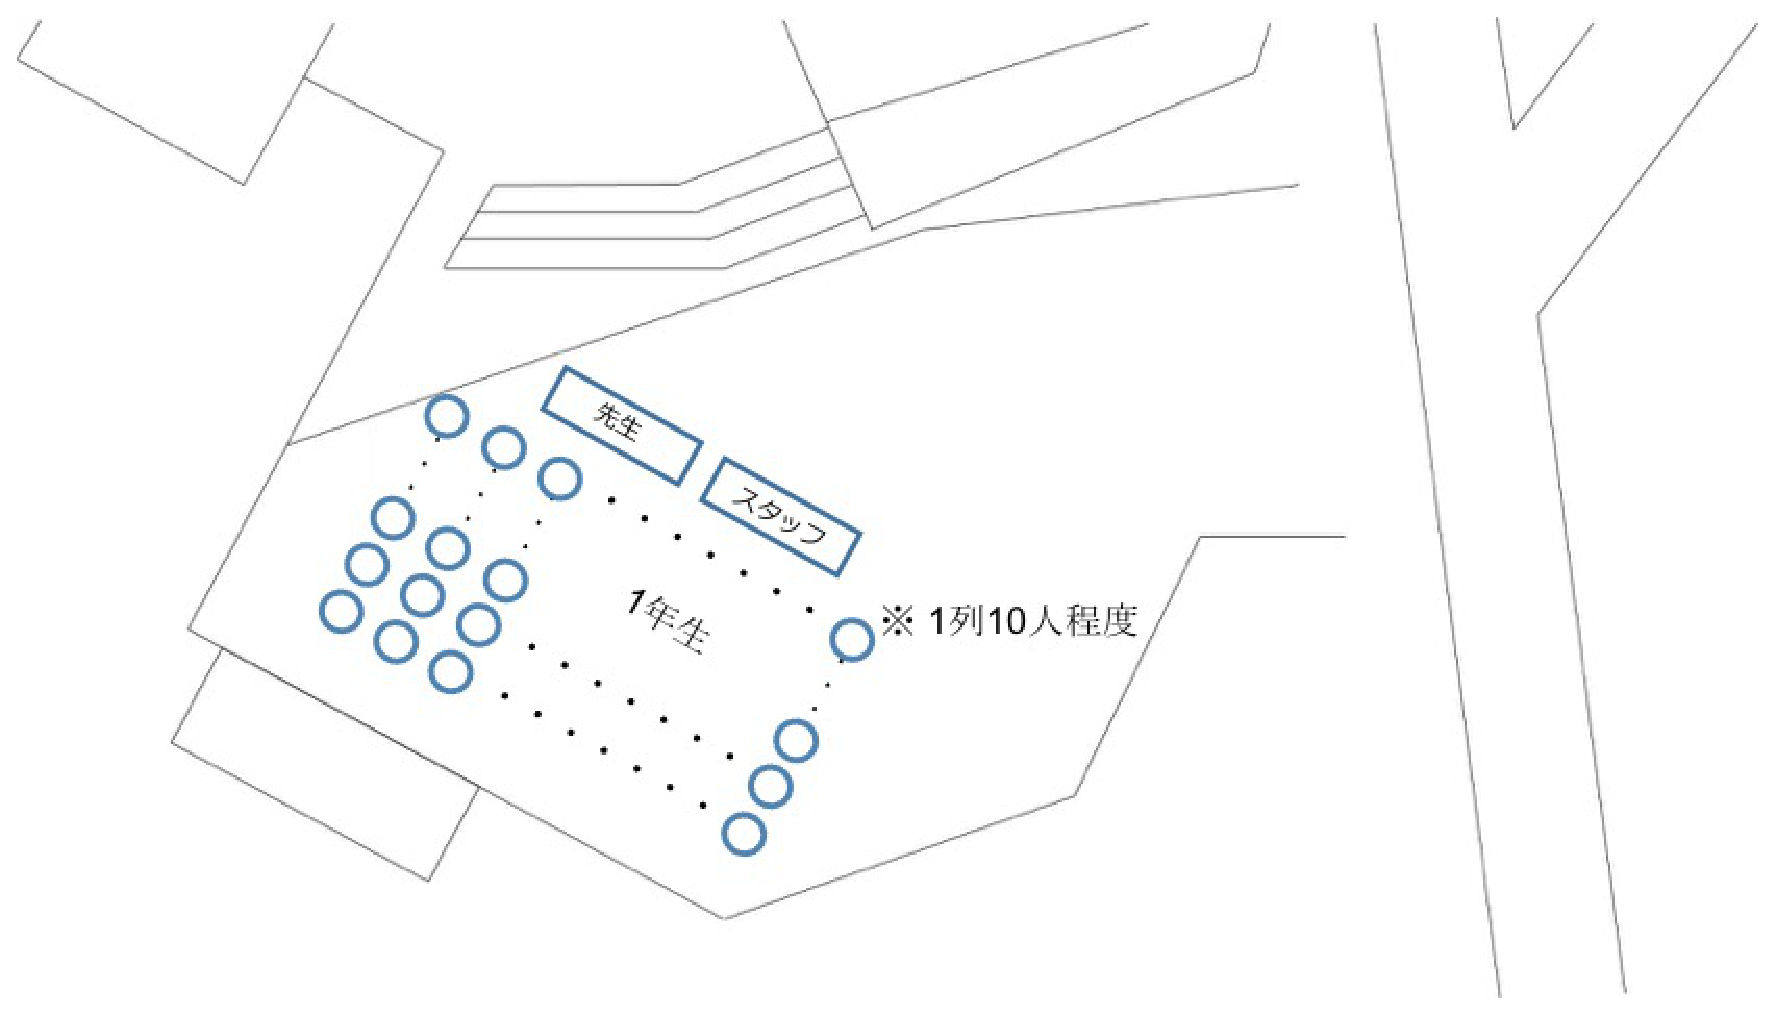
\includegraphics[width = 11cm]{./17/asanotudoihaiti.eps}
\caption{正面広間}
\end{center}
\end{figure}


\subsection{朝のつどいから食堂までの誘導位置}
\begin{figure}[h]
\begin{center}
  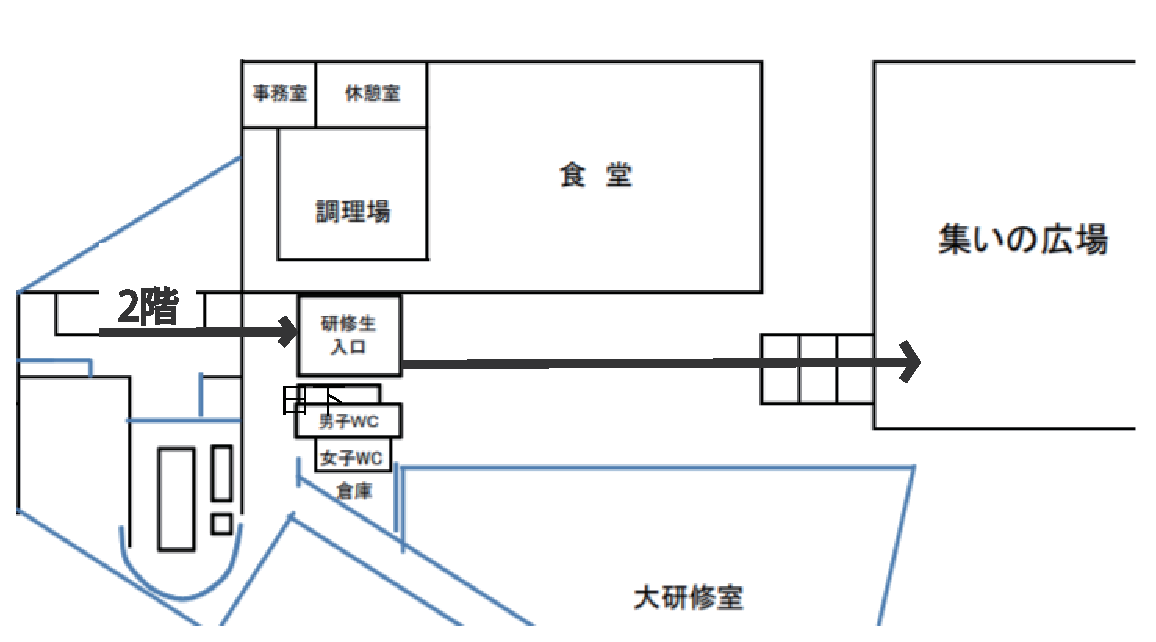
\includegraphics[width = 16cm]{./17/asanozu.eps}
\end{center}
\end{figure}


%\subsection{備考}
%人員に入っていないスタッフも朝の集いに参加する

%\subsection{連絡事項}
%\begin{table}[htb]
%\begin{tabular}{|l|c|c|} \hline
%報告者 & 内容 & タイミング \\ \hline \hline
 %& くろしお棟1誘導開始 & 7:10(誘導開始時)  \\ \hline
 %&  くろしお棟2誘導開始 & くろしお棟1退出後 \\ \hline
 %&  くろしお棟3誘導開始 & くろしお棟2退出後  \\ \hline
 %&  くろしお棟4誘導開始 & くろしお棟3退出後 \\ \hline
 %&  食堂へ誘導開始 & 自身のスタッフ代表挨拶終了後 \\ \hline

%\end{tabular}
%\end{table}

%\include{end}
